\documentclass[10pt]{article}
\usepackage[margin=1.0cm]{geometry}
\usepackage[T1]{fontenc}
\usepackage{lmodern}
\usepackage{xcolor}
\usepackage{tikz}
\usepackage{pgfplots}
\usepgfplotslibrary{statistics}
\pgfplotsset{compat=1.18}
\definecolor{srblue}{HTML}{2F6B9A}
\definecolor{opencvorange}{HTML}{D97706}
\definecolor{fps2blue}{HTML}{B9D7EA}
\definecolor{fps5orange}{HTML}{F6C28B}
\definecolor{stslightgreen}{HTML}{A7D8B1}
\definecolor{stsstronggreen}{HTML}{208B3A}
\definecolor{sugarlightpurple}{HTML}{CBB7E8}
\definecolor{sugarstrongpurple}{HTML}{763A9B}
\definecolor{stsedge}{HTML}{1D4E89}
\definecolor{sugaredge}{HTML}{B45309}
\definecolor{incompletegray}{HTML}{9CA3AF}
\definecolor{deltared}{HTML}{B91C1C}
\definecolor{deltagreen}{HTML}{15803D}
\begin{document}
\pagestyle{empty}
\begin{center}
{\Large\bfseries Bildmetriken im Verhältnis zur Laufzeit}\\[3pt]
{\small Explorative Darstellung; Laufzeit = vollständiger archivierter Pipeline-Lauf}\\[8pt]
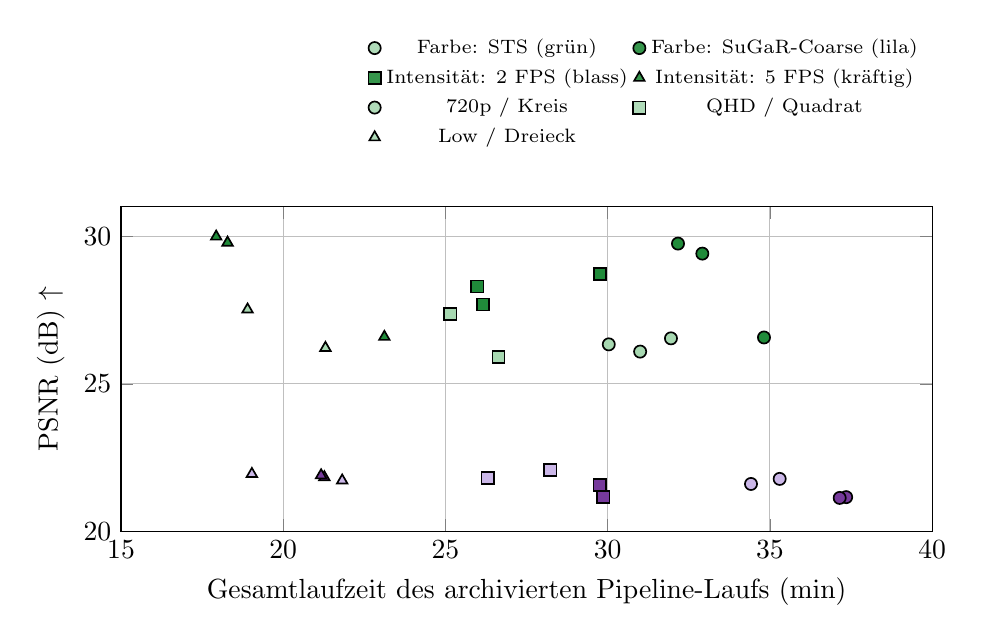
\begin{tikzpicture}
\begin{axis}[width=0.98\linewidth,height=5.7cm,xlabel={Gesamtlaufzeit des archivierten Pipeline-Laufs (min)},ylabel={PSNR (dB) $\uparrow$},xmin=15,xmax=40,xtick={15,20,25,30,35,40},ymin=20,ymax=31,grid=major,legend style={font=\scriptsize,at={(1.0,1.15)},anchor=south east,draw=none,fill=white,fill opacity=0.9,text opacity=1},legend columns=2]
\addplot[only marks,mark=*,mark size=2.2pt,mark options={fill=stslightgreen,draw=black,line width=0.6pt}] coordinates {(30.033333,26.33820363)};
\addplot[only marks,mark=*,mark size=2.2pt,mark options={fill=stsstronggreen,draw=black,line width=0.6pt}] coordinates {(32.916667,29.41639448)};
\addplot[only marks,mark=square*,mark size=2.2pt,mark options={fill=stsstronggreen,draw=black,line width=0.6pt}] coordinates {(25.983333,28.29924453)};
\addplot[only marks,mark=triangle*,mark size=2.2pt,mark options={fill=stsstronggreen,draw=black,line width=0.6pt}] coordinates {(18.283333,29.78896627)};
\addplot[only marks,mark=*,mark size=2.2pt,mark options={fill=stslightgreen,draw=black,line width=0.6pt}] coordinates {(31.000000,26.09251831)};
\addplot[only marks,mark=square*,mark size=2.2pt,mark options={fill=stslightgreen,draw=black,line width=0.6pt}] coordinates {(25.150000,27.36821420)};
\addplot[only marks,mark=triangle*,mark size=2.2pt,mark options={fill=stslightgreen,draw=black,line width=0.6pt}] coordinates {(18.900000,27.51974000)};
\addplot[only marks,mark=*,mark size=2.2pt,mark options={fill=stsstronggreen,draw=black,line width=0.6pt}] coordinates {(32.166667,29.75600052)};
\addplot[only marks,mark=square*,mark size=2.2pt,mark options={fill=stsstronggreen,draw=black,line width=0.6pt}] coordinates {(26.150000,27.68839292)};
\addplot[only marks,mark=triangle*,mark size=2.2pt,mark options={fill=stsstronggreen,draw=black,line width=0.6pt}] coordinates {(17.933333,29.99353907)};
\addplot[only marks,mark=*,mark size=2.2pt,mark options={fill=stslightgreen,draw=black,line width=0.6pt}] coordinates {(31.950000,26.54214463)};
\addplot[only marks,mark=square*,mark size=2.2pt,mark options={fill=stslightgreen,draw=black,line width=0.6pt}] coordinates {(26.633333,25.91712114)};
\addplot[only marks,mark=triangle*,mark size=2.2pt,mark options={fill=stslightgreen,draw=black,line width=0.6pt}] coordinates {(21.300000,26.21822335)};
\addplot[only marks,mark=*,mark size=2.2pt,mark options={fill=stsstronggreen,draw=black,line width=0.6pt}] coordinates {(34.816667,26.57282792)};
\addplot[only marks,mark=square*,mark size=2.2pt,mark options={fill=stsstronggreen,draw=black,line width=0.6pt}] coordinates {(29.766667,28.71943249)};
\addplot[only marks,mark=triangle*,mark size=2.2pt,mark options={fill=stsstronggreen,draw=black,line width=0.6pt}] coordinates {(23.116667,26.59301839)};
\addplot[only marks,mark=*,mark size=2.2pt,mark options={fill=sugarlightpurple,draw=black,line width=0.6pt}] coordinates {(34.416667,21.60365263)};
\addplot[only marks,mark=square*,mark size=2.2pt,mark options={fill=sugarlightpurple,draw=black,line width=0.6pt}] coordinates {(26.300000,21.80344288)};
\addplot[only marks,mark=triangle*,mark size=2.2pt,mark options={fill=sugarlightpurple,draw=black,line width=0.6pt}] coordinates {(19.033333,21.94173862)};
\addplot[only marks,mark=*,mark size=2.2pt,mark options={fill=sugarstrongpurple,draw=black,line width=0.6pt}] coordinates {(37.350000,21.15583377)};
\addplot[only marks,mark=square*,mark size=2.2pt,mark options={fill=sugarstrongpurple,draw=black,line width=0.6pt}] coordinates {(29.750000,21.57142085)};
\addplot[only marks,mark=triangle*,mark size=2.2pt,mark options={fill=sugarstrongpurple,draw=black,line width=0.6pt}] coordinates {(21.266667,21.83137436)};
\addplot[only marks,mark=*,mark size=2.2pt,mark options={fill=sugarlightpurple,draw=black,line width=0.6pt}] coordinates {(35.300000,21.77515639)};
\addplot[only marks,mark=square*,mark size=2.2pt,mark options={fill=sugarlightpurple,draw=black,line width=0.6pt}] coordinates {(28.233333,22.08118374)};
\addplot[only marks,mark=triangle*,mark size=2.2pt,mark options={fill=sugarlightpurple,draw=black,line width=0.6pt}] coordinates {(21.816667,21.72007820)};
\addplot[only marks,mark=*,mark size=2.2pt,mark options={fill=sugarstrongpurple,draw=black,line width=0.6pt}] coordinates {(37.150000,21.12995336)};
\addplot[only marks,mark=square*,mark size=2.2pt,mark options={fill=sugarstrongpurple,draw=black,line width=0.6pt}] coordinates {(29.866667,21.16734883)};
\addplot[only marks,mark=triangle*,mark size=2.2pt,mark options={fill=sugarstrongpurple,draw=black,line width=0.6pt}] coordinates {(21.166667,21.89677851)};
\addlegendimage{only marks,mark=*,mark size=2.2pt,mark options={fill=stsstronggreen,draw=black}}\addlegendentry{Farbe: STS (grün)}
\addlegendimage{only marks,mark=*,mark size=2.2pt,mark options={fill=sugarstrongpurple,draw=black}}\addlegendentry{Farbe: SuGaR-Coarse (lila)}
\addlegendimage{only marks,mark=*,mark size=2.2pt,mark options={fill=stslightgreen,draw=black}}\addlegendentry{Intensität: 2 FPS (blass)}
\addlegendimage{only marks,mark=*,mark size=2.2pt,mark options={fill=stsstronggreen,draw=black}}\addlegendentry{Intensität: 5 FPS (kräftig)}
\addlegendimage{only marks,mark=*,mark size=2.2pt,mark options={fill=white,draw=black}}\addlegendentry{720p / Kreis}
\addlegendimage{only marks,mark=square*,mark size=2.2pt,mark options={fill=white,draw=black}}\addlegendentry{QHD / Quadrat}
\addlegendimage{only marks,mark=triangle*,mark size=2.2pt,mark options={fill=white,draw=black}}\addlegendentry{Low / Dreieck}
\end{axis}\end{tikzpicture}\par\vspace{2pt}
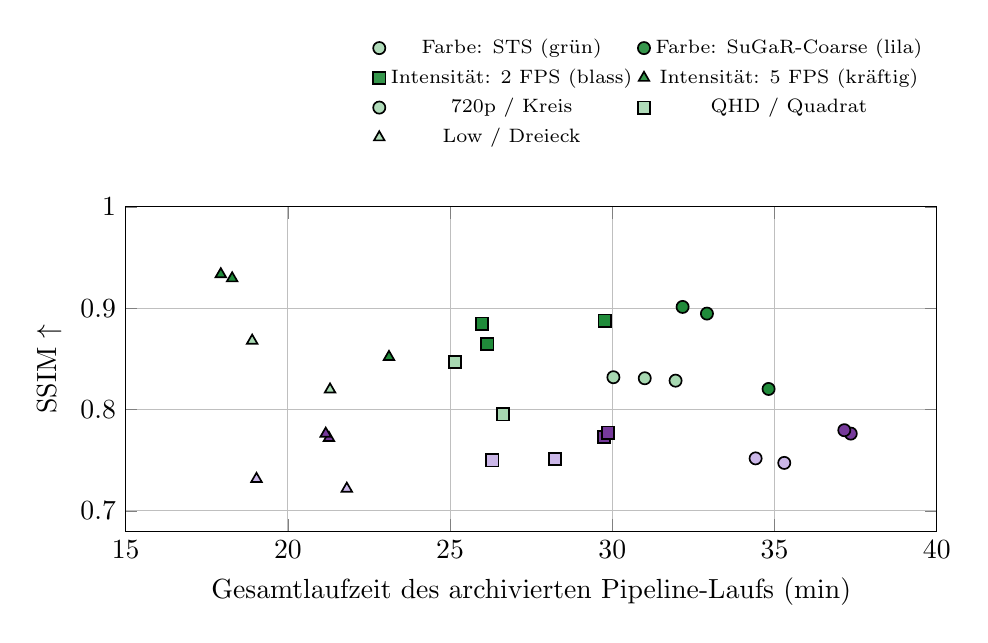
\begin{tikzpicture}
\begin{axis}[width=0.98\linewidth,height=5.7cm,xlabel={Gesamtlaufzeit des archivierten Pipeline-Laufs (min)},ylabel={SSIM $\uparrow$},xmin=15,xmax=40,xtick={15,20,25,30,35,40},ymin=0.68,ymax=1.0,grid=major,legend style={font=\scriptsize,at={(1.0,1.15)},anchor=south east,draw=none,fill=white,fill opacity=0.9,text opacity=1},legend columns=2]
\addplot[only marks,mark=*,mark size=2.2pt,mark options={fill=stslightgreen,draw=black,line width=0.6pt}] coordinates {(30.033333,0.83195574)};
\addplot[only marks,mark=*,mark size=2.2pt,mark options={fill=stsstronggreen,draw=black,line width=0.6pt}] coordinates {(32.916667,0.89474248)};
\addplot[only marks,mark=square*,mark size=2.2pt,mark options={fill=stsstronggreen,draw=black,line width=0.6pt}] coordinates {(25.983333,0.88487382)};
\addplot[only marks,mark=triangle*,mark size=2.2pt,mark options={fill=stsstronggreen,draw=black,line width=0.6pt}] coordinates {(18.283333,0.92957129)};
\addplot[only marks,mark=*,mark size=2.2pt,mark options={fill=stslightgreen,draw=black,line width=0.6pt}] coordinates {(31.000000,0.83093130)};
\addplot[only marks,mark=square*,mark size=2.2pt,mark options={fill=stslightgreen,draw=black,line width=0.6pt}] coordinates {(25.150000,0.84708937)};
\addplot[only marks,mark=triangle*,mark size=2.2pt,mark options={fill=stslightgreen,draw=black,line width=0.6pt}] coordinates {(18.900000,0.86803825)};
\addplot[only marks,mark=*,mark size=2.2pt,mark options={fill=stsstronggreen,draw=black,line width=0.6pt}] coordinates {(32.166667,0.90132959)};
\addplot[only marks,mark=square*,mark size=2.2pt,mark options={fill=stsstronggreen,draw=black,line width=0.6pt}] coordinates {(26.150000,0.86479931)};
\addplot[only marks,mark=triangle*,mark size=2.2pt,mark options={fill=stsstronggreen,draw=black,line width=0.6pt}] coordinates {(17.933333,0.93359960)};
\addplot[only marks,mark=*,mark size=2.2pt,mark options={fill=stslightgreen,draw=black,line width=0.6pt}] coordinates {(31.950000,0.82856342)};
\addplot[only marks,mark=square*,mark size=2.2pt,mark options={fill=stslightgreen,draw=black,line width=0.6pt}] coordinates {(26.633333,0.79535064)};
\addplot[only marks,mark=triangle*,mark size=2.2pt,mark options={fill=stslightgreen,draw=black,line width=0.6pt}] coordinates {(21.300000,0.81985135)};
\addplot[only marks,mark=*,mark size=2.2pt,mark options={fill=stsstronggreen,draw=black,line width=0.6pt}] coordinates {(34.816667,0.82038200)};
\addplot[only marks,mark=square*,mark size=2.2pt,mark options={fill=stsstronggreen,draw=black,line width=0.6pt}] coordinates {(29.766667,0.88779274)};
\addplot[only marks,mark=triangle*,mark size=2.2pt,mark options={fill=stsstronggreen,draw=black,line width=0.6pt}] coordinates {(23.116667,0.85198560)};
\addplot[only marks,mark=*,mark size=2.2pt,mark options={fill=sugarlightpurple,draw=black,line width=0.6pt}] coordinates {(34.416667,0.75188178)};
\addplot[only marks,mark=square*,mark size=2.2pt,mark options={fill=sugarlightpurple,draw=black,line width=0.6pt}] coordinates {(26.300000,0.74990743)};
\addplot[only marks,mark=triangle*,mark size=2.2pt,mark options={fill=sugarlightpurple,draw=black,line width=0.6pt}] coordinates {(19.033333,0.73163200)};
\addplot[only marks,mark=*,mark size=2.2pt,mark options={fill=sugarstrongpurple,draw=black,line width=0.6pt}] coordinates {(37.350000,0.77630728)};
\addplot[only marks,mark=square*,mark size=2.2pt,mark options={fill=sugarstrongpurple,draw=black,line width=0.6pt}] coordinates {(29.750000,0.77305094)};
\addplot[only marks,mark=triangle*,mark size=2.2pt,mark options={fill=sugarstrongpurple,draw=black,line width=0.6pt}] coordinates {(21.266667,0.77199414)};
\addplot[only marks,mark=*,mark size=2.2pt,mark options={fill=sugarlightpurple,draw=black,line width=0.6pt}] coordinates {(35.300000,0.74740580)};
\addplot[only marks,mark=square*,mark size=2.2pt,mark options={fill=sugarlightpurple,draw=black,line width=0.6pt}] coordinates {(28.233333,0.75128989)};
\addplot[only marks,mark=triangle*,mark size=2.2pt,mark options={fill=sugarlightpurple,draw=black,line width=0.6pt}] coordinates {(21.816667,0.72197089)};
\addplot[only marks,mark=*,mark size=2.2pt,mark options={fill=sugarstrongpurple,draw=black,line width=0.6pt}] coordinates {(37.150000,0.77968981)};
\addplot[only marks,mark=square*,mark size=2.2pt,mark options={fill=sugarstrongpurple,draw=black,line width=0.6pt}] coordinates {(29.866667,0.77716404)};
\addplot[only marks,mark=triangle*,mark size=2.2pt,mark options={fill=sugarstrongpurple,draw=black,line width=0.6pt}] coordinates {(21.166667,0.77627132)};
\addlegendimage{only marks,mark=*,mark size=2.2pt,mark options={fill=stsstronggreen,draw=black}}\addlegendentry{Farbe: STS (grün)}
\addlegendimage{only marks,mark=*,mark size=2.2pt,mark options={fill=sugarstrongpurple,draw=black}}\addlegendentry{Farbe: SuGaR-Coarse (lila)}
\addlegendimage{only marks,mark=*,mark size=2.2pt,mark options={fill=stslightgreen,draw=black}}\addlegendentry{Intensität: 2 FPS (blass)}
\addlegendimage{only marks,mark=*,mark size=2.2pt,mark options={fill=stsstronggreen,draw=black}}\addlegendentry{Intensität: 5 FPS (kräftig)}
\addlegendimage{only marks,mark=*,mark size=2.2pt,mark options={fill=white,draw=black}}\addlegendentry{720p / Kreis}
\addlegendimage{only marks,mark=square*,mark size=2.2pt,mark options={fill=white,draw=black}}\addlegendentry{QHD / Quadrat}
\addlegendimage{only marks,mark=triangle*,mark size=2.2pt,mark options={fill=white,draw=black}}\addlegendentry{Low / Dreieck}
\end{axis}\end{tikzpicture}\par\vspace{2pt}
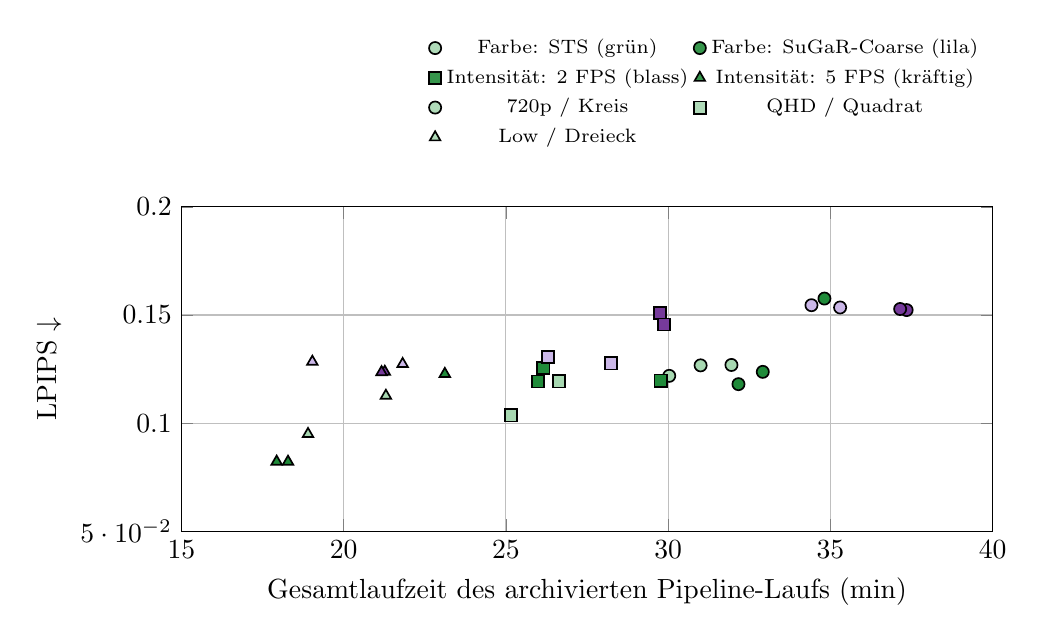
\begin{tikzpicture}
\begin{axis}[width=0.98\linewidth,height=5.7cm,xlabel={Gesamtlaufzeit des archivierten Pipeline-Laufs (min)},ylabel={LPIPS $\downarrow$},xmin=15,xmax=40,xtick={15,20,25,30,35,40},ymin=0.05,ymax=0.2,grid=major,legend style={font=\scriptsize,at={(1.0,1.15)},anchor=south east,draw=none,fill=white,fill opacity=0.9,text opacity=1},legend columns=2]
\addplot[only marks,mark=*,mark size=2.2pt,mark options={fill=stslightgreen,draw=black,line width=0.6pt}] coordinates {(30.033333,0.12186836)};
\addplot[only marks,mark=*,mark size=2.2pt,mark options={fill=stsstronggreen,draw=black,line width=0.6pt}] coordinates {(32.916667,0.12371773)};
\addplot[only marks,mark=square*,mark size=2.2pt,mark options={fill=stsstronggreen,draw=black,line width=0.6pt}] coordinates {(25.983333,0.11927220)};
\addplot[only marks,mark=triangle*,mark size=2.2pt,mark options={fill=stsstronggreen,draw=black,line width=0.6pt}] coordinates {(18.283333,0.08216407)};
\addplot[only marks,mark=*,mark size=2.2pt,mark options={fill=stslightgreen,draw=black,line width=0.6pt}] coordinates {(31.000000,0.12672276)};
\addplot[only marks,mark=square*,mark size=2.2pt,mark options={fill=stslightgreen,draw=black,line width=0.6pt}] coordinates {(25.150000,0.10358845)};
\addplot[only marks,mark=triangle*,mark size=2.2pt,mark options={fill=stslightgreen,draw=black,line width=0.6pt}] coordinates {(18.900000,0.09497066)};
\addplot[only marks,mark=*,mark size=2.2pt,mark options={fill=stsstronggreen,draw=black,line width=0.6pt}] coordinates {(32.166667,0.11802495)};
\addplot[only marks,mark=square*,mark size=2.2pt,mark options={fill=stsstronggreen,draw=black,line width=0.6pt}] coordinates {(26.150000,0.12551100)};
\addplot[only marks,mark=triangle*,mark size=2.2pt,mark options={fill=stsstronggreen,draw=black,line width=0.6pt}] coordinates {(17.933333,0.08218506)};
\addplot[only marks,mark=*,mark size=2.2pt,mark options={fill=stslightgreen,draw=black,line width=0.6pt}] coordinates {(31.950000,0.12690219)};
\addplot[only marks,mark=square*,mark size=2.2pt,mark options={fill=stslightgreen,draw=black,line width=0.6pt}] coordinates {(26.633333,0.11930196)};
\addplot[only marks,mark=triangle*,mark size=2.2pt,mark options={fill=stslightgreen,draw=black,line width=0.6pt}] coordinates {(21.300000,0.11265756)};
\addplot[only marks,mark=*,mark size=2.2pt,mark options={fill=stsstronggreen,draw=black,line width=0.6pt}] coordinates {(34.816667,0.15761947)};
\addplot[only marks,mark=square*,mark size=2.2pt,mark options={fill=stsstronggreen,draw=black,line width=0.6pt}] coordinates {(29.766667,0.11964402)};
\addplot[only marks,mark=triangle*,mark size=2.2pt,mark options={fill=stsstronggreen,draw=black,line width=0.6pt}] coordinates {(23.116667,0.12276925)};
\addplot[only marks,mark=*,mark size=2.2pt,mark options={fill=sugarlightpurple,draw=black,line width=0.6pt}] coordinates {(34.416667,0.15454567)};
\addplot[only marks,mark=square*,mark size=2.2pt,mark options={fill=sugarlightpurple,draw=black,line width=0.6pt}] coordinates {(26.300000,0.13049116)};
\addplot[only marks,mark=triangle*,mark size=2.2pt,mark options={fill=sugarlightpurple,draw=black,line width=0.6pt}] coordinates {(19.033333,0.12839596)};
\addplot[only marks,mark=*,mark size=2.2pt,mark options={fill=sugarstrongpurple,draw=black,line width=0.6pt}] coordinates {(37.350000,0.15229463)};
\addplot[only marks,mark=square*,mark size=2.2pt,mark options={fill=sugarstrongpurple,draw=black,line width=0.6pt}] coordinates {(29.750000,0.15094676)};
\addplot[only marks,mark=triangle*,mark size=2.2pt,mark options={fill=sugarstrongpurple,draw=black,line width=0.6pt}] coordinates {(21.266667,0.12377006)};
\addplot[only marks,mark=*,mark size=2.2pt,mark options={fill=sugarlightpurple,draw=black,line width=0.6pt}] coordinates {(35.300000,0.15349434)};
\addplot[only marks,mark=square*,mark size=2.2pt,mark options={fill=sugarlightpurple,draw=black,line width=0.6pt}] coordinates {(28.233333,0.12767535)};
\addplot[only marks,mark=triangle*,mark size=2.2pt,mark options={fill=sugarlightpurple,draw=black,line width=0.6pt}] coordinates {(21.816667,0.12735538)};
\addplot[only marks,mark=*,mark size=2.2pt,mark options={fill=sugarstrongpurple,draw=black,line width=0.6pt}] coordinates {(37.150000,0.15278799)};
\addplot[only marks,mark=square*,mark size=2.2pt,mark options={fill=sugarstrongpurple,draw=black,line width=0.6pt}] coordinates {(29.866667,0.14565088)};
\addplot[only marks,mark=triangle*,mark size=2.2pt,mark options={fill=sugarstrongpurple,draw=black,line width=0.6pt}] coordinates {(21.166667,0.12357728)};
\addlegendimage{only marks,mark=*,mark size=2.2pt,mark options={fill=stsstronggreen,draw=black}}\addlegendentry{Farbe: STS (grün)}
\addlegendimage{only marks,mark=*,mark size=2.2pt,mark options={fill=sugarstrongpurple,draw=black}}\addlegendentry{Farbe: SuGaR-Coarse (lila)}
\addlegendimage{only marks,mark=*,mark size=2.2pt,mark options={fill=stslightgreen,draw=black}}\addlegendentry{Intensität: 2 FPS (blass)}
\addlegendimage{only marks,mark=*,mark size=2.2pt,mark options={fill=stsstronggreen,draw=black}}\addlegendentry{Intensität: 5 FPS (kräftig)}
\addlegendimage{only marks,mark=*,mark size=2.2pt,mark options={fill=white,draw=black}}\addlegendentry{720p / Kreis}
\addlegendimage{only marks,mark=square*,mark size=2.2pt,mark options={fill=white,draw=black}}\addlegendentry{QHD / Quadrat}
\addlegendimage{only marks,mark=triangle*,mark size=2.2pt,mark options={fill=white,draw=black}}\addlegendentry{Low / Dreieck}
\end{axis}\end{tikzpicture}\par\vspace{2pt}
\vspace{3pt}
\begin{minipage}{0.98\linewidth}\scriptsize Die x-Achse zeigt die vollständige Dauer des archivierten Pipeline-Laufs zwischen Start und Ende in \texttt{run.md}; ältere Berichte ohne Start/Ende verwenden ersatzweise die Summe ihrer aufgezeichneten Schritte. SAM3/COLMAP sind nur enthalten, sofern sie innerhalb dieses archivierten Laufs lagen. Die Darstellung ist explorativ und kein Geometrie-Qualitätsranking.\end{minipage}
\end{center}
\end{document}